\documentclass[12pt]{article}
%\documentclass[11pt]{report}
\usepackage{./styles/daves,fancyhdr,natbib,url}
\usepackage{amsmath}
\usepackage{amssymb}
\usepackage{graphicx}
\usepackage{pdfpages}
\usepackage{lscape}
\usepackage{booktabs}
\usepackage{dcolumn}
\usepackage{paralist}

%%%%%%%%%% Will's stuff BELOW %%%%%%%
\usepackage[left=1.25in, right=1.25in,
            top=1in, bottom=1in]{geometry}                % See geometry.pdf to learn the layout options. There are lots.
\geometry{letterpaper}

\usepackage{ragged2e}

\usepackage{xcolor}
\newcommand{\codeRcolor}{0.93}
\newcommand{\codeGcolor}{0.93}
\newcommand{\codeBcolor}{0.93}
\definecolor{lightgrey}{rgb}{\codeRcolor,
                             \codeGcolor,
                             \codeBcolor}

\newcommand{\listingfont}{\fontsize{7pt}{8pt}\selectfont\ttfamily}
\usepackage{listings}
\lstset{basicstyle = \listingfont,
        breaklines = true,
        frame=tb,
        xleftmargin=12pt,
        framexleftmargin=6pt,
        framexrightmargin=6pt,
        xrightmargin=12pt,
        columns=fixed}
\lstset{lineskip=-1pt}
\lstset{backgroundcolor=\color{lightgrey}}


\usepackage[font={footnotesize},
            labelfont={sf,bf},
            textfont={sf},
            singlelinecheck=false,
            labelsep=none,
            justification=RaggedRight,
            aboveskip=0pt,
            belowskip=7pt plus 1pt minus 1pt,
            textformat=period]{caption}
\DeclareCaptionLabelSeparator{mystyle}{.\quad}
\captionsetup{labelsep=mystyle}
%%%%%%%%% Will's Stuff ABOVE %%%%%%%%%

\cfoot{\thepage}


\thispagestyle{plain}
%\bibliographystyle{./styles/chicago}
%\bibliographystyle{apalike}



\begin{document}
%%%%%%%%%% COVER %%%%%%%%%%%%
\begingroup
\begin{center}
\textbf{CE 5366 Water Resources Management}\\{Concepts and Tools for Decision Making}
\end{center}
%%%%%%
\begin{figure}[htbp] %  figure placement: here, top, bottom, or page
   \centering
   \includegraphics[width=6in]{./support/drops-of-water-water-nature-liquid-40784-e1481152386844.jpg} 
%   \caption{example caption}
   \label{fig:example}
\end{figure}
%%%%%%



\begin{center}
by \\
Theodore G. Cleveland \\
Department of Civil, Environmental, and Construction Engineering \\
Texas Tech University\\
~\\
January 2018 \\
\end{center}
\endgroup
~\\
~\\
~\\
~\\
~\\
~\\
~\\
Suggested citation: Cleveland, T. G. 2018. ``Water Resources Management; Concepts and Tools for Decision Making." 
CE 5366 Lecture Notes, Department of Civil, Environmental, and Construction Engineering, Texas Tech University.
\clearpage
%%%%%%%%%%%%%%%%%%%%%%%%%%%
\tableofcontents
\section{Introduction}
words
\subsection{What is Water Resources Management?}
Water resources management is:
\begin{quote}The activity of planning, developing, distributing and managing the optimum use of water
resources. Water resource management planning considers the competing demands for/
on water (quantity, quality, location, and timing) and seeks to allocate water on an
equitable basis to satisfy all uses and demands.
\end{quote}

Paraphrasing WRSPM:
\begin{quote}
The central purpose of water resources planning and management activities is to
address and, if possible, answer questions such as:\\
How can renewable yet finite water resources (e.g. rivers, estuaries, lakes, glaciers, and coastal zones) best be managed and used?
How can this management and use be accomplished in an environment of uncertain supplies and uncertain and increasing demands, and consequently of increasing conflicts among individuals having different interests in the management of a river and its basin?
\end{quote}

Key concepts/terms are
\begin{itemize}
\item Finite (limited) water resource.
\item How much, when, how yummy.
\item Allocate to many.
\item Equity/conflicts.
\item ``Best be managed $\dots$''
\end{itemize}
\newpage
\subsubsection{What is ``Allocate''}
Allocate means \\~\\
1: to apportion for a specific purpose or to particular persons or things : distribute
allocate tasks among human and automated components\\
2: to set apart or earmark : designate allocate a section of the building for special
research purposes\\

If the resource is abundant then allocation is unnecessary.  
However, water resources are identified as finite, hence limited in scope both spatially and temporally.

Because the resource is scarce; allocation will necessarily deny the resource to some, and supply it to others.

\subsubsection{What is ``Equitable''}
Equitable means \\~\\
1: having or exhibiting equity : dealing fairly and equally with all concerned an
equitable settlement of the dispute \\
2: existing or valid in equity as distinguished from law an equitable defense\\

Because the resource is scarce; allocation will necessarily deny the resource
to some, and supply it to others. 
Equity implies some kind of ?fairness? in that allocation.

\subsection{Decision Making}
The allocation requires decisions be made.
Decisions (policy) may involve the activity of an individual decision maker or collective decision maker(s).
These two classifications may make decisions quite differently, based on their roles, emotions, and goals.

\subsubsection{How do individuals and groups make decisions?}
Some people may seem indecisive or inconsistent. 
They may avoid making decisions as long as possible.
The same reluctance to make decisions also happens in organizations or institutions.
The decision avoidance may be an individual or collective desire to address uncertainty, in waiting, more information may become available.

On the other hand, some people and groups may be accused of ``jumping to conclusions" or making a decision ``without considering all the facts."
The decision acceleration may be an individual or collective assessment of the utility of more information, or a value judgement of the importance of the actual situation to longer term goals, or acknowledgement of urgency, or just plain laziness -- all of these explanations are clearly situational dependent.

This dichotomy itself contains a valuable implication that, in general, decisions should be made by collecting and weighing various elements in a rational way. 
Furthermore, alternatives must exist, or there is no decision to make.   

Decision making contains deep psychological aspects. People's choices depend upon how alternatives are
presented -- consider Figure \ref{fig:Picture1.png}.
\begin{figure}[h!] %  figure placement: here, top, bottom, or page
   \centering
   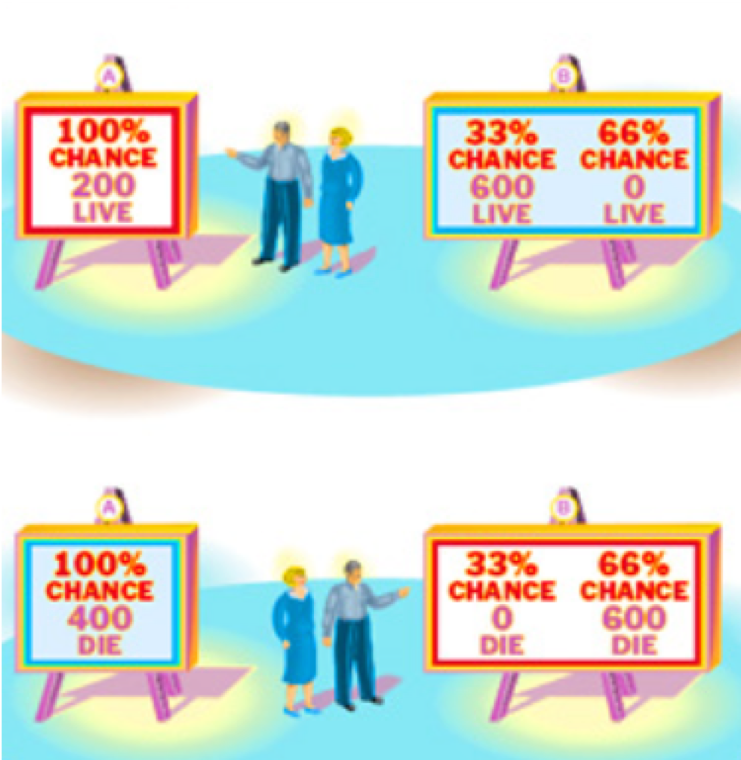
\includegraphics[width=6in]{./Lesson1/Picture1.png} 
   \caption{Identical decisions.  Upper panel is "Survival Based"; Lower panel is "Mortality Based" }
   \label{fig:Picture1.png}
\end{figure}
\newline
Consider the decision A or B,  the actual outcomes in terms of probability and number of survivors of the decision.\\
If we make decision A. The probability $P$ of the outcomes are $P(S=200) = \frac{1}{1}; P(S=0) = \frac{0}{1}$.
If we make decision B. The probability $P$ of the outcomes are  $P(S=600) = \frac{1}{3}; P(S=0) = \frac{2}{3}$.

Expectation in this structure is the product of the value of the outcome and the probability of that outcome.
Thus $E(S_A) = 1.0 \times 200 + 0.0 \times 0 = 200~\text{people}$, and  $E(S_B) = \frac{1}{3} \times 600 + \frac{2}{3} \times 0 =  200~\text{people}$.

Whichever decision is chosen A or B has the same expected outcome (in terms of expectation in the statistical sense); 200 people survive.
So one might conclude it does not matter which decision we make -- but that's not the whole story.  

While decision A guarantees 200 survive, decision B has a 66\% chance or zero survivors -- which is intended here to illustrate the influence of uncertainty in decision making.

Furthermore, how the situation is presented (Survival Based or Mortality Based) can have a severe emotional influence on how one would make the choice.

Lastly, consider the exogenous influences.  If the people in the example pay taxes, then the cost of the decision could influence the actual decision.

This simple example illustrates the challenges of something seemingly as simple as making a decision.

\subsection{Challenge of Water Resources Management}
There are actually only a few challenges (at a very high cognitive level):
\begin{itemize}
\item Define alternatives (present decision points)
\item Define value
\item Define outcomes
\item Define equity; ``what is fair'' for a situation
\item Implement tools to support (defend) the decision
\item Implement the decision(s)
\end{itemize}

\subsubsection{Support Tools}
One of the bullet items is tools to support the decision.  
These include economics or some other way to value the alternatives (cost and benefit), as well as measure ``fairness''
Then some policy (or procedure) to rank the value(s).
Another policy or procedure to guide the decision -- in some instances we could hand off the decision to an algorithm (Narrow Domain AI).  We already let such algorithms fly aircraft with us in them, recommend products for us to purchase, detect fraudulent fiscal activity and such.
Another important factor in the support/implementation component is what level of control do we have.
\begin{itemize}
\item Do we control the system? \\
SCADA operating a water distribution network -- fully autonomous with little human intervention.
%Autopilot algorithm to operate a commercial aircraft -- fully autonomous with little human intervention.
\item $\dots$ or just influence the system \\
Voluntary compliance versus risk of apprehension for water quality management
\end{itemize}

%\subsubsection{Example}
%\subsection{Assigning Value}
%\subsubsection{Example}
%\subsection{Readings}
%\subsection{Exercises}
\section{Engineering Economy}
words
\subsection{Time Value of Money}
\subsubsection{Example}
\subsection{Comparing Alternatives}
\subsubsection{Example}
\subsection{Perspective}
\subsubsection{Example}
\subsection{Readings}
\subsection{Exercises}
\include{./Lesson3/Lesson3}
\include{./Lesson4/Lesson4}
\include{./Lesson5/Lesson5}
\include{./Lesson6/Lesson6}
\include{./Lesson7/Lesson7}
\section{Simulation Tools - A Decision Consequence Estimation Component}
The purpose of a simulation in the context of this document is to predict the response of a system to the decisions; that is what is the anticipated state of the system after the decisions have been applied.  Did the decisions improve the situation, or make it worse, or no detectable change.
\subsection{Simulation and Models}
define a model



\subsubsection{Example}
\subsection{Statistical Models}
\subsubsection{Example}
\subsection{Analog Models}
Analog models are models where analogs of the real system to be studied are employed.
Column, Jar, and bench-scale studies in Environmental Engineering are examples of analog (and physical) models of a real system.
Flume and estuary  scale physical models are examples of analog (and scaled) models of a real system.
Electric circuit analogs have been built to simulate behavior of river systems and groundwater aquifers -- actual instances of these kinds of models are today only likely to be found in museums; computer models have largely replaced these kind of analog models.

In general analog models are outside the scope of this document, they are useful, they are expensive, and they are uncommon (with the exception of the Environmental Engineering laboratory models).
\subsubsection{Example}
\subsection{Digital Models}
\subsubsection{Example}
Use an on-line network simulator to make a decision.  
\subsection{Readings}
\subsection{Exercises}
\include{./Lesson9/Lesson9}
\include{./Lesson10/Lesson10}
\include{./Lesson11/Lesson11} % Multi-Stage LP
\include{./Lesson12/Lesson12}
\include{./Lesson13/Lesson13}
\include{./Lesson14/Lesson14}
\include{./Lesson15/Lesson15}
\include{./Lesson16/Lesson16}
\include{./Lesson17/Lesson17}
\include{./Lesson18/Lesson18}
\include{./Lesson19/Lesson19}
\include{./Lesson20/Lesson20}
\include{./Lesson21/Lesson21}
\include{./Lesson22/Lesson22}
\include{./Lesson23/Lesson23}
\section{Title}
words
\subsection{Topic 1}
\subsubsection{Example}
\subsection{Topic 2}
\subsubsection{Example}
\subsection{Topic 3}
\subsubsection{Example}
\subsection{Readings}
\subsection{Exercises}


%%%%%%%%%% INTRODUCTION %%%%%%%%%%
%\section{Problem Statement}
%
%Figure \ref{} is a plan-view picture of a confined aquifer that has the shape of a square 10 km $\times$ 10km.
%Three sides of the aquifer have impermeable boundaries, the fourth side is a lake into which the aquifer drains.
%
%The lake water quality is poor, and to keep lake water from entering the aquifer minimum water levels in the aquifer along the lake are to be maintained.  
%These water levels are +0.64 m above the lake level in cells 21 through 25, and +0.95 m above the lake level in cells 16 through 20.
%
%The aquifer is recharged from rainfall that passes through the upper confining bed at a rate of $N=100$ mm/yr, uniformly distributed over the entire area.  Under natural conditions the entire recharge is drained through the aquifer to the lake.  The aquifer is homogeneous with transmissivity $T=1000~m^2/day$.
%
%Each cell in the diagram is to be considered a single point where pumping may occur (within that cell).  
%
%A consumer is located in cell 18 which represents the location of water demand -- all water pumped is routed to this center for use.
%The total water demand of the one consumer is $D = 7\times10^{6}~m^3/yr$. 
%The cost to pump and transport water from Cell 18 to the consumer is $ \$1.0/m^3 $.
%The cost increases with distance from the pumping area in Cell 18 at a rate of $ \frac{\$0.5/m^3}{1000m \text{~distance}}$.
%
%Determine a least-cost steady flow pumping strategy to supply the required demand and maintain the required water levels in the aquifer.
%\section{Solution Approach}
%The problem requires the ability to estimate the impact of pumping on the aquifer -- that is for a particular pumping strategy the engineer needs to be able to determine the water levels at each cell in the aquifer and check these against the minimum requires levels -- the simulation component.
%
%The problem also requires a way to select among different pumping strategies that if feasible (the simulation results satisfy the minimum water levels), are lowest cost -- the optimization component.
%
%The decisions to be made are the amount of pumping in each cell, and the total cost is computed from knowing which cells have non-zero pumping and multiplying these values by the price for pumping and transmission from that cell the to demand center.
%
%\subsection{Linear Programming Model Framework}
%[Cost for each cell]
%[demand constraint]
%[influence constraints]
%
%%\include{16-PorousMediumFlow/PorousMediumFlow}
%\include{17-SteadyGroundwaterFlow/SteadyGroundwaterFlow}
%\section{Solving the Simulation-Optimization Problem}
%Script to build the LP and solve it.
%
%


%%%%%%%%%%
%\clearpage
%See my stuff in Listing~\ref{lst:pre}.

%% Ted, one major difficulty in using captions for listings as shown here is that commas are used as an argument delimiter. If you require the use of the comma in a caption you will have to surrounded with braces as shown for the listing in example 1.  TeX will throw an error if you try to typeset it otherwise.

%\begin{lstlisting}[caption=R code demonstrating, label=lst:pre]
%txdot0_6654.db <- read.table("database_txdot0-6654.txt",
%                             header=TRUE, sep="|")
%DB <- txdot0_6654.db; # shorten the database name considerably

%"weibullpp" <- function(x, sort=TRUE) {
%    denom <- length(x) + 1
%    ranks <- rank(x, ties.method = "first")
%    ifelse(sort, return((sort(ranks))/denom), return((ranks)/denom))
%}
%XLAB  <- "NONEXCEEDANCE PROBABILITY"
%YLABV <- "VELOCITY, IN FEET PER SECOND"
%YLABQ <- "DISCHARGE, IN CUBIC FEET PER SECOND"
%\end{lstlisting}

%

%\begin{lstlisting}[caption=R code that needs a comma{,} in the caption{,} but remember that references to other listings can be made like this Listing~\ref{lst:pre}{,} which is responsible for setting up these examples, label=lst:exam1]
%# EXAMPLE 1
%#   ** Empirical Distribution of Discharge
%# Get all measurements for watershed area less than 1000 square miles and compute
%# the 50th percentile using the quantile() function of R---this is the median
%Q <- DB[DB$CDA < 1000, ]$Q; # condition as explained, note the comma
%print(quantile(Q, 0.5))     # compute and show, 22.2 cubic feet per second
%#>  50%
%#> 22.2
%\end{lstlisting}

%
%\begin{lstlisting}[caption=R code demonstrating, label=lst:exam2]
%# EXAMPLE 2
%#   ** Empirical Distribution of Mean Velocity
%# Get all mean velocities for which the cross-sectional area is greater than
%# 100 square feet and less than 5000 square feet. Also, want mean annual precipitation
%# greater than 30 inches and watershed area less than 750 square miles. Finally, want
%# to filter for discharges greater than the 60th percentile for the flow-duration curve
%# a the station. Again note the use of the comma, which is critical and the & means "and"
%DD  <- DB[DB$A > 100 & DB$A < 5000, ]; # cross section area: 100 <= A <= 5000
%VEL <- DD[DD$CDA < 750 & DD$MAP > 30 & DD$FDC > 0.60, ]$V; # watershed and flow prob.
%plot(weibullpp(VEL), sort(VEL), type="l", xlab=XLAB, ylab=YLABV, lwd=2)
%\end{lstlisting}

%
%\begin{lstlisting}[caption=R code demonstrating, label=lst:exam3]
%# EXAMPLE 3
%#   ** Empirical Distribution of Discharge
%# Get all measurements for watershed area less than 100 square miles
%#   and topwidth less than 40 feet
%#   and greater than 80th percentile on the flow-duration curve
%# Compute the 75th percentile of these measurements
%print(quantile(DB[DB$CDA < 100 & DB$B < 40 & DB$FDC > 0.80, ]$Q, 0.75))
%#>   75%
%#> 75.35
%# Solution is 75 cubic feet per second, coincidence that two "75s" show up.

%\end{lstlisting}
%%%%%%%%%%%%


\begin{thebibliography}{3}


%
\bibitem[Asquith and Slade(1997)]{AS1997}
Asquith, W.H., and Slade, R.M., 1997, Regional equations for estimation of peak-streamflow frequency for natural basins in Texas: U.S. Geological Survey Water Resources Investigations Report 96--4307, \url{http://pubs.usgs.gov/wri/wri964307/}.

\bibitem[Asquith, and Roussel (2009)]{AR2009}
Asquith, W.H., and Roussel, M. S., 2009, Regression equations for estimation of annual peak-streamflow frequency for undeveloped watershed in Texas using an L-moment-based, PRESS-minimized, residual adjusted approach. U.S. Geological Survey Scientific Investigations Report 2009--5087.

\bibitem[Asquith, Herrmann, and Cleveland(2013)]{AsquithQVGAM2013}
Asquith, W.H., Herrmann, G.R., and Cleveland, T.G., 2013, Use of generalized additive modeling for regionalization of a discharge measurement database in Texas. Journal of Hydrologic Engineering, American Society of Civil Engineers, \textsl{in press}
%
\bibitem[Gordon and others(2004)]{Gordon2004}
Gordon, N.D., T.A. McMahon, B.L. Finlayson, C.J. Gippel, R.J. Nathan, 2004,
Stream Hydrology: An Introduction for Ecologists (second edition). John Wiley, The Atrium, Southern Gate, Chichester, West Sussex PO19 8SQ,
England, 429~p.

%
%\bibitem[Homer and other(2004)]{Homer2004}
%Homer, C., Huang, C., Yang, L., Wylie, B., and Coan, M., 2004, Development of a 2001 national land cover database for the United States: Photogrammetric Engineering and Remote Sensing, v.~70, no.~7, p. 829--840, \url{http://www.mrlc.gov/nlcd2001.php}.

%\bibitem[Miller(1953)]{Miller1953}
%Miller, V.C., 1953, A quantitative geomorphic study of drainage basin
%characteristics in the Clinch Mountain area, Virginia and Tennessee: Columbia
%University, Department of Geology, Technical Report, no.~3, Contract N6-ONR
%271--300. [Miller proposed the circular ratio for expressing characteristics of basin shape.]

%\bibitem[Strahler(1952)]{Strahler1952}
%Strahler, A.N. 1952, Dynamic basis of geomorphology: Bulletin of the Geological Society of America, 63:923--938.

%\bibitem[Shreve(1967)]{Shreve1967}
%Shreve, R.L. 1967. Infinite topologically random channel networks: Journal of
%Geology, 75:178--186.


\bibitem[USGS(2009)]{NWISmeasurements}
U.S. Geological Survey, 2009, Streamflow measurements for Texas: USGS National Water Information System, accessed March 1, 2009, \url{http://waterdata.usgs.gov/tx/nwis/measurements/?site_no=STATIONID&agency_cd=USGS}.

%\bibitem[USGS(2009b)]{NWISdv}
%U.S. Geological Survey, 2009b, Daily mean streamflow values for Texas: USGS National Water Information System, accessed March 1, 2009, \url{http://waterdata.usgs.gov/tx/nwis/dv/?site_no=STATIONID&agency_cd=USGS}

\end{thebibliography}



\end{document}




